\documentclass{beamer}
\usepackage[utf8]{inputenc}
\usepackage[T2A,T1]{fontenc}
\usepackage[english, russian]{babel}
\usetheme{Pittsburgh}

\selectlanguage{russian}
\newcommand{\define}[2]{{\bf #1} --- #2\vspace{1em}}
\newcommand{\longdef}[1]{{\textbf{\underline{Опр:}} #1}}
\newcommand{\set}[1]{{\lbrace #1 \rbrace}}

\title{Симметричная криптография. Блочные шифры}
\institute{ВГУ}
\date{2014}
\begin{document}

\frame{\titlepage}

\begin{frame}
  \frametitle{Классификация криптографических алгоритмов}

  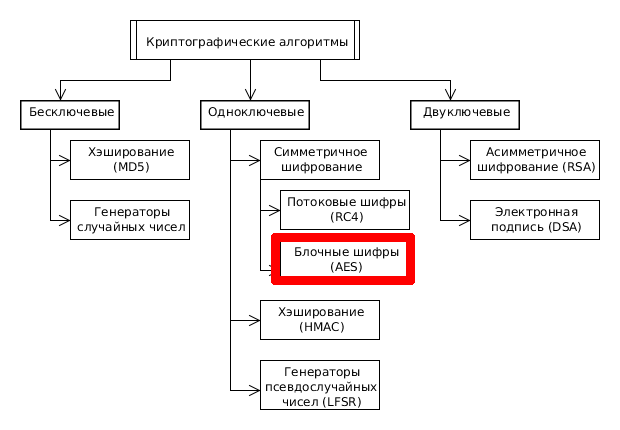
\includegraphics[width=\linewidth]{./images/png/CA_classification_block.png}

\end{frame}

\begin{frame}
  \frametitle{Потоковые шифры}

  \begin{itemize}
    \itemsep 2em
    \item{Основная идея: замена потока действительно случайных чисел на 
      поток псевдослучайных чисел}
    \item{$G$ - генератор псевдослучайных чисел}
    \item{Функция шифрования: \newline
      $E(k,m)=m \oplus G(k)$}
    \item{Функция дешифрования: \newline
      $D(k,c)=c \oplus G(k)$}
    \item{Может применяться к сообщениям произвольной длины}
  \end{itemize}

\end{frame}


\begin{frame}
  \frametitle{Недостатки потоковых шифров}

  \begin{itemize}
    \itemsep 2em
    \item{Невозможность использования одинаковых значений ключа дважды}
    \item{Невозможность проверки целостности сообщений}
    \item{Состояние ГСЧ на обоих сторонах общения должно быть синхронизировано}
    \item{Результат шифрования полностью определяется открытым текстом и
      используемым ключом}
  \end{itemize}

\end{frame}


\begin{frame}
  \frametitle{Определение}

  \define{Блочный шифр (block cipher)} {функция шифрования, которая применяется к блокам текста фиксированной длины}
  

  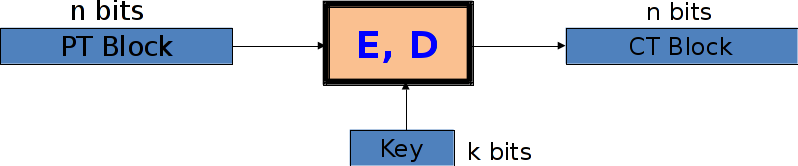
\includegraphics[width=\linewidth]{images/png/block_cipher_overview.png}

  \vspace{1em}

  \textbf{AES}: n=128 bits, k = 128, 192, 256

  \note{Шифр принимает на вход n-битный открытый текст и выдает n-битный шифрованный текст}
  \note{Открытый и шифрованный текст всегда имеет один и тот же размер, который называется размером блока}
  \note{Рассказать о том, насколько блочные шифры важны и случаи, когда нам нужно шифровать именно блоками, а не потоком.
        Поточные шифры являются state-full алгоритмами, в отличие от блочных шифров. Поточные шифры плохо подходят когда
        приходится использовать ключ несколько раз (шифрование файлов), а также когда используются message-oriented
        протоколы}
  \note{Блочные шифры намного медленнее, чем потоковые. Можно взять слайд 3 у Boneh}

\end{frame}


\begin{frame}
  \frametitle{Основные принципы работы}

  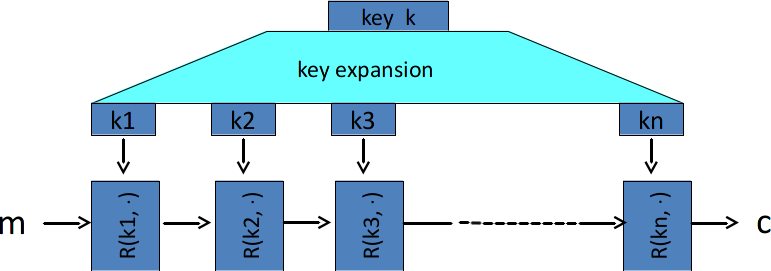
\includegraphics[width=\linewidth]{images/png/work_principle.png}

  \vspace{1em}

  $R(k,m)$ - раундовая функция

  У AES-128 10 раундовых функций
  \note{The idea is to make a strong encryption function out of a weaker
        round function (easy to implement) by repeatedly using it.}
  \note{For every subkey the round function must be invertible; if not
        decryption is impossible.}
\end{frame}


\begin{frame}
  \frametitle{Псевдослучайные функции и перестановки}

  \define{Псевдослучайная функция (Pseudo Random Function, PRF)}
    {эффективно вычислимая функция, определенная на $(K,X,Y)$ \newline
    \[F: K \times X \rightarrow Y\]}

\end{frame}


\begin{frame}
  \frametitle{Псевдослучайные функции и перестановки}

  \define{Псевдослучайная перестановка (Pseudo Random Permutation, PRP)}
    {эффективно вычислимая функция, определенная на $(K,X)$ \newline
    \[E: K \times X \rightarrow X\]
    и имеющая следующие свойства:

    \begin{itemize}
      \item{Существует эффективно вычислимый алгоритм для вычисления $E(k,x)$}
      \item{Функция $E(k,\cdot)$ является однозначной}
      \item{Существует эффективно вычислимый алгоритм для нахождения обратной функции $D(k,y)$}
    \end{itemize}
  }

  \note{Нарисовать отображение, задаваемое перестановкой и подчеркнуть однозначность функции.
    Однозначность функции позволяет задать функцию дешифрования.}
  \note{Понятия PRP и блочный шифр являются взаимозаменяемыми.}
  \note{Любая PRP является PRF. 2 отличия - X отображается само на себя и существует обратная однозначная функция}

\end{frame}


\begin{frame}
  \frametitle{Безопасные PRF}

  \begin{block}{Интуитивное определение безопасности PRF}

  $F: K \times X \rightarrow Y$ - некоторая PRF

  \vspace{1em}
  Определим:
  \begin{displaymath}
    \left\{
      \begin{array}{l}
        Funs[X,Y]:\textnormal{ множество всех возможных функций из $X$ в $Y$} \\
        \note{Это не PRF. Здесь нет параметра k. Просто все возможные дискретные функции из X в Y}
        S_{F} = \set{ F(k, \cdot), k \in K} \subset Funs[X,Y]
      \end{array}
    \right.
  \end{displaymath}

  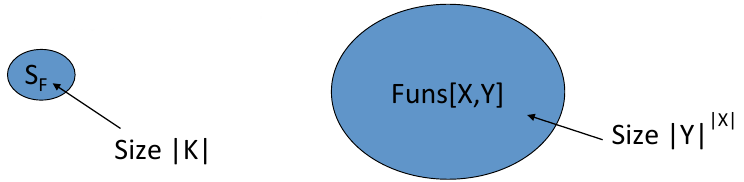
\includegraphics[width=\linewidth]{images/png/PRF_set.png}

  Невозможно отличить случайно выбранную функцию из $Funs[X,Y]$ от функции, случайно выбранной из $S_{F}$ 
  \end{block}

\end{frame}


\begin{frame}
  \frametitle{Безопасные PRF}

  \begin{block}{Пример использования}

  $F: K \times \set{0,1}^{n} \rightarrow \set{0,1}^{n}$ - безопасная PRF

  \vspace{1em}
  Построим безопасный ГСЧ на основе $F$
  \vspace{1em}

  $G: K \rightarrow \set{0,1}^{nt}$

  \[G(k) = F(k,0) || F(k,1) ||  \ldots || F(k,t) \]

  \note{Главное достоинство такого генератора - возможность распараллеливания на несколько процессоров. Так как
   безопасный ГСЧ даёт нам напрямую потоковый шифр, то мы получаем пример параллельного потокового шифра}
  \note{Безопасность ГСЧ основана на том, что $F(k,x)$ неотличима от действительно случайной $f(x)$}
  \end{block}

\end{frame}


\begin{frame}
  \frametitle{Основные принципы работы}

  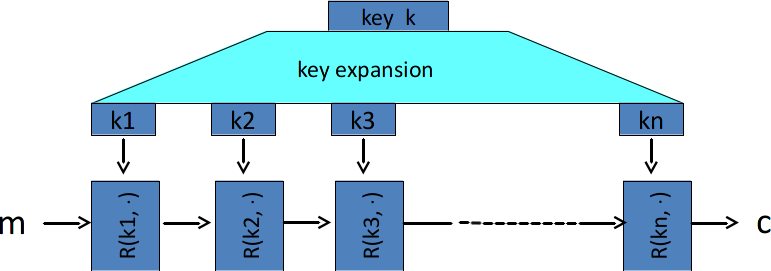
\includegraphics[width=\linewidth]{images/png/work_principle.png}

  \vspace{1em}

  $R(k,m)$ - раундовая функция

  У AES-128 10 раундовых функций
\end{frame}


\begin{frame}
  \frametitle{AES}

  \begin{block}{История}
    \begin{itemize}
      \item{1997: NIST начал прием заявок на новый стандарт шифрования для замены DES}
      \item{1998: Было предложено на рассмотрение 15 заявок}
      \item{1999: NIST выбрало 5 финалистов}
      \item{2000: NIST утвердило шифр Rijndael в качестве нового стандарта (AES)}
    \end{itemize}
  \end{block}

  \begin{block}{Характеристики}
    \begin{itemize}
      \item{Размеры ключей: 128, 192, 256 бит}
      \item{Размер блока: 128 бит}
    \end{itemize}
  \end{block}
\end{frame}

\begin{frame}
  \frametitle{Принцип работы AES}

  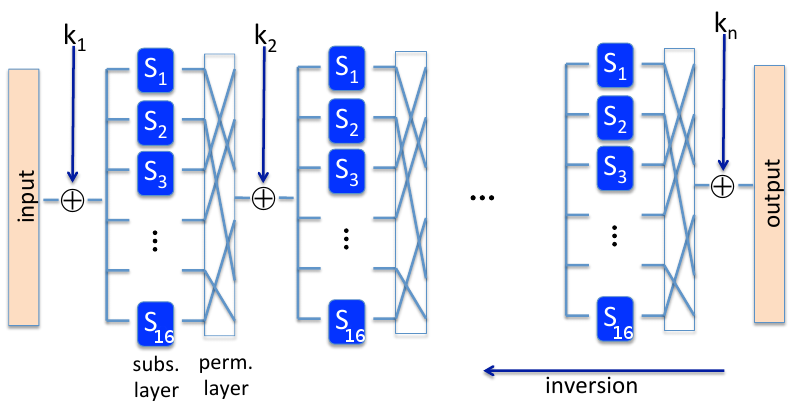
\includegraphics[width=\linewidth]{images/png/AES_network}
\end{frame}


\begin{frame}
  \frametitle{Принцип работы AES}

  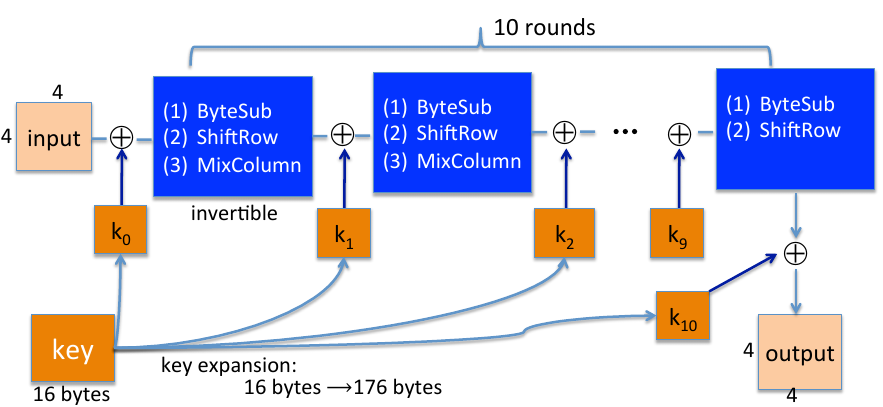
\includegraphics[width=\linewidth]{images/png/AES_rounds}
\end{frame}

\begin{frame}
  \frametitle{Принцип работы AES}

  \begin{block}{Раундовая функция}
    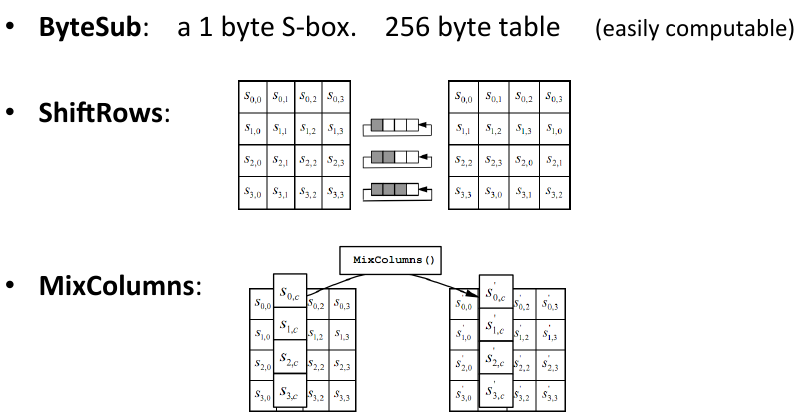
\includegraphics[width=\linewidth]{images/png/AES_round_function}
  \end{block}

\end{frame}


\begin{frame}
  \frametitle{Реализация алгоритма AES}

  \begin{block}{Выбор между скоростью работы и занимаемой памятью}
    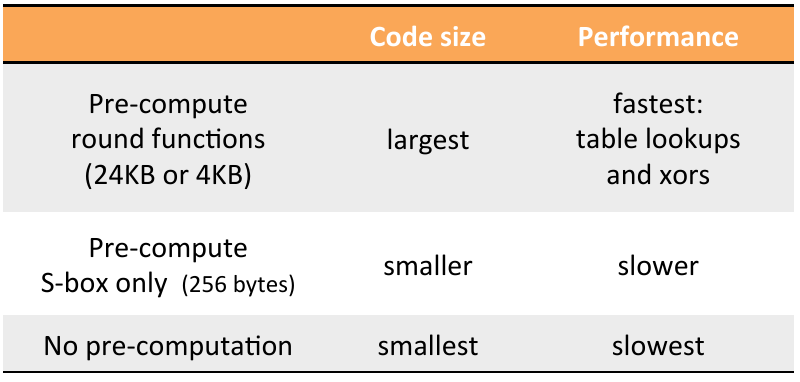
\includegraphics[width=\linewidth]{images/png/AES_implementation_tradeoff}
  \end{block}

  \note{Trade-off between size and speed}
  \note{Существуют специальные ассемблерные инструкции для архитектуры x86, которые реализуют алгоритм AES}
\end{frame}


\begin{frame}
  \frametitle{Построение PRF на основе ГСЧ}

  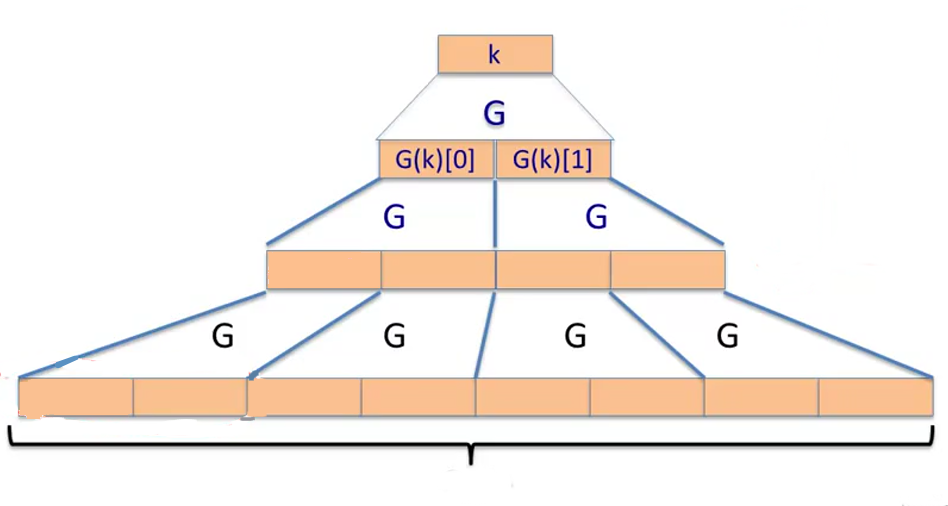
\includegraphics[width=\linewidth]{images/png/prf_from_prg}

\end{frame}


\note{Доказать безопасность AES более-менее формально тяжело, потому что в алгоритме
используется большое количество эвристик. Хотелось бы построить блочный шифр из примитивов, которые сами по себе
безопасны. Такие примитивы - безопасные ГСЧ}

%TODO: Slides for building block ciphers from PRG
%TODO: Add slides for solving problems of ECB mode


\begin{frame}
  \frametitle{Режим шифрования ECB (Шифрование независимыми блоками)}

  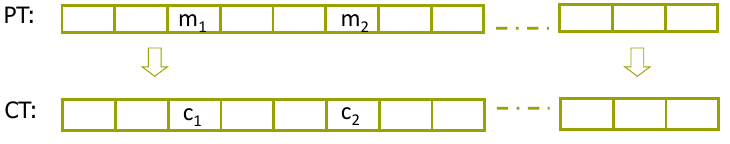
\includegraphics[width=\linewidth]{images/png/ECB_mode}

  \begin{itemize}
    \item{ECB -- пример некорректного использования PRP}
    \item{Основная проблема: если $m_{1}=m_{2}$, то $c_{1}=c_{2}$}
  \end{itemize}

\end{frame}


\begin{frame}
  \frametitle{Режим шифрования ECB (Шифрование независимыми блоками)}

  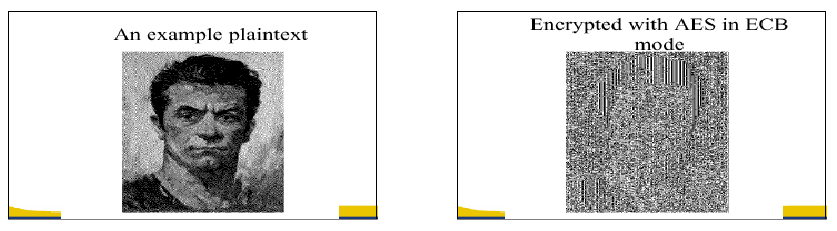
\includegraphics[width=\linewidth]{images/png/ECB_failure}

\end{frame}


\begin{frame}
  \frametitle{Детерминированный режим счетчика (Det CTR)}

  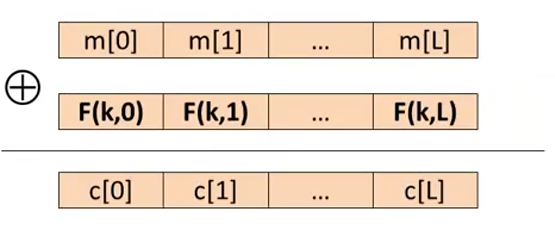
\includegraphics[width=\linewidth]{images/png/deterministic_CTR}

\end{frame}

%TODO: Refine slides for CBC and CTR modes

\begin{frame}
  \frametitle{Алгоритм создания цепочек CBC}

  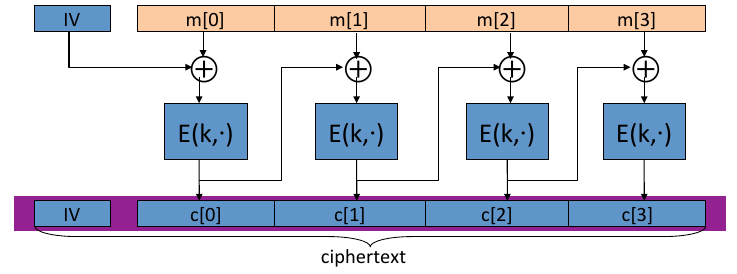
\includegraphics[width=\linewidth]{images/png/CBC_random_IV}

\end{frame}


\begin{frame}
  \frametitle{Алгоритм создания цепочек CTR}

  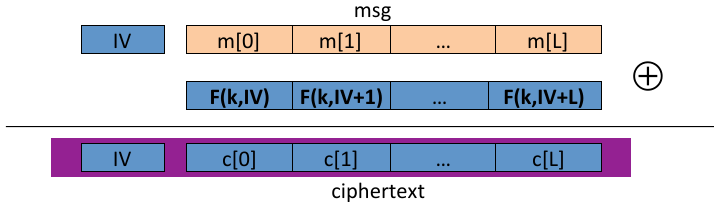
\includegraphics[width=\linewidth]{images/png/CTR_mode}

\end{frame}


\begin{frame}
  \frametitle{Сравнение алгоритмов CBC и CTR}

  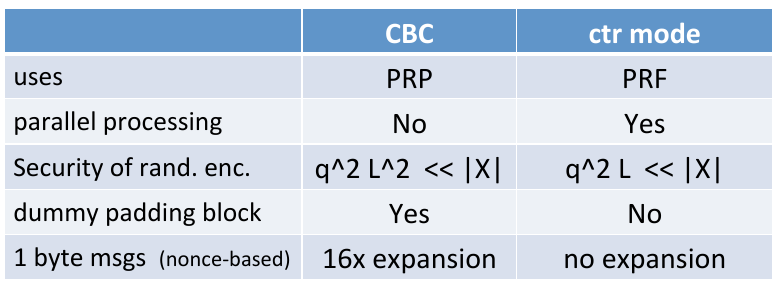
\includegraphics[width=\linewidth]{images/png/CTR_vs_CBC_comparison}

\end{frame}

\end{document}
